% Options for packages loaded elsewhere
\PassOptionsToPackage{unicode}{hyperref}
\PassOptionsToPackage{hyphens}{url}
%
\documentclass[
]{article}
\usepackage{amsmath,amssymb}
\usepackage{iftex}
\ifPDFTeX
  \usepackage[T1]{fontenc}
  \usepackage[utf8]{inputenc}
  \usepackage{textcomp} % provide euro and other symbols
\else % if luatex or xetex
  \usepackage{unicode-math} % this also loads fontspec
  \defaultfontfeatures{Scale=MatchLowercase}
  \defaultfontfeatures[\rmfamily]{Ligatures=TeX,Scale=1}
\fi
\usepackage{lmodern}
\ifPDFTeX\else
  % xetex/luatex font selection
\fi
% Use upquote if available, for straight quotes in verbatim environments
\IfFileExists{upquote.sty}{\usepackage{upquote}}{}
\IfFileExists{microtype.sty}{% use microtype if available
  \usepackage[]{microtype}
  \UseMicrotypeSet[protrusion]{basicmath} % disable protrusion for tt fonts
}{}
\makeatletter
\@ifundefined{KOMAClassName}{% if non-KOMA class
  \IfFileExists{parskip.sty}{%
    \usepackage{parskip}
  }{% else
    \setlength{\parindent}{0pt}
    \setlength{\parskip}{6pt plus 2pt minus 1pt}}
}{% if KOMA class
  \KOMAoptions{parskip=half}}
\makeatother
\usepackage{xcolor}
\usepackage[margin=1in]{geometry}
\usepackage{longtable,booktabs,array}
\usepackage{calc} % for calculating minipage widths
% Correct order of tables after \paragraph or \subparagraph
\usepackage{etoolbox}
\makeatletter
\patchcmd\longtable{\par}{\if@noskipsec\mbox{}\fi\par}{}{}
\makeatother
% Allow footnotes in longtable head/foot
\IfFileExists{footnotehyper.sty}{\usepackage{footnotehyper}}{\usepackage{footnote}}
\makesavenoteenv{longtable}
\usepackage{graphicx}
\makeatletter
\def\maxwidth{\ifdim\Gin@nat@width>\linewidth\linewidth\else\Gin@nat@width\fi}
\def\maxheight{\ifdim\Gin@nat@height>\textheight\textheight\else\Gin@nat@height\fi}
\makeatother
% Scale images if necessary, so that they will not overflow the page
% margins by default, and it is still possible to overwrite the defaults
% using explicit options in \includegraphics[width, height, ...]{}
\setkeys{Gin}{width=\maxwidth,height=\maxheight,keepaspectratio}
% Set default figure placement to htbp
\makeatletter
\def\fps@figure{htbp}
\makeatother
\setlength{\emergencystretch}{3em} % prevent overfull lines
\providecommand{\tightlist}{%
  \setlength{\itemsep}{0pt}\setlength{\parskip}{0pt}}
\setcounter{secnumdepth}{-\maxdimen} % remove section numbering
\ifLuaTeX
  \usepackage{selnolig}  % disable illegal ligatures
\fi
\usepackage{bookmark}
\IfFileExists{xurl.sty}{\usepackage{xurl}}{} % add URL line breaks if available
\urlstyle{same}
\hypersetup{
  pdftitle={Tundra Light Extinction Model},
  pdfauthor={Ruby An},
  hidelinks,
  pdfcreator={LaTeX via pandoc}}

\title{Tundra Light Extinction Model}
\author{Ruby An}
\date{2024-01-12}

\begin{document}
\maketitle

\section{Introduction}\label{introduction}

This document describes a multi-species model of tundra plant community
dynamics. The goals of this model are to:

\begin{enumerate}
\def\labelenumi{(\alph{enumi})}
\tightlist
\item
  explain the coexistence of multiple species in tundra plant
  communities, and
\item
  make predictions about community-level outcomes in a changing climate.
\end{enumerate}

Our approach is to build a simple model informed by the physical
structure, demographic processes, and resource requirements common to
plant species in tundra environments. We characterize equilibrium
dynamics of the model and establish criterion for species coexistence as
a function of species' traits.

We then test how environmental change (warming, longer growing seasons,
higher nutrient availability) alters competitive outcomes through a
series of simulations. Environmental conditions alter outcomes by
impacting species' growth rates, time available for growth, and
mortality risk.

\section{Model Description}\label{model-description}

This model tracks the density of ramets (\(X_{i}\) -- the number of
individual ramets of species \(i\) in a given unit area) in continuous
time. For ease of notation, we order species from tallest to shortest
ramet height:

\[ H_{1} > H_{2} > \cdots > H_{j} > H_{i} > \cdots > H_{Q} \text{ for species } i = 1, 2, ..., Q   \]
In this imagination of the tundra world, ramets never ``grow in
height'', but are instantaneously born at their species-specific height
once a ``mother ramet'' has accumulated enough carbon. This means that
each species occupies only one specific height \(H_i\) in the canopy at
any given point in time. This simplifies the description of the light
environment, such that we are able to easily calculate equilibrium
environmental conditions, ramet densities, and coexistence criterion.

\begin{figure}
\centering
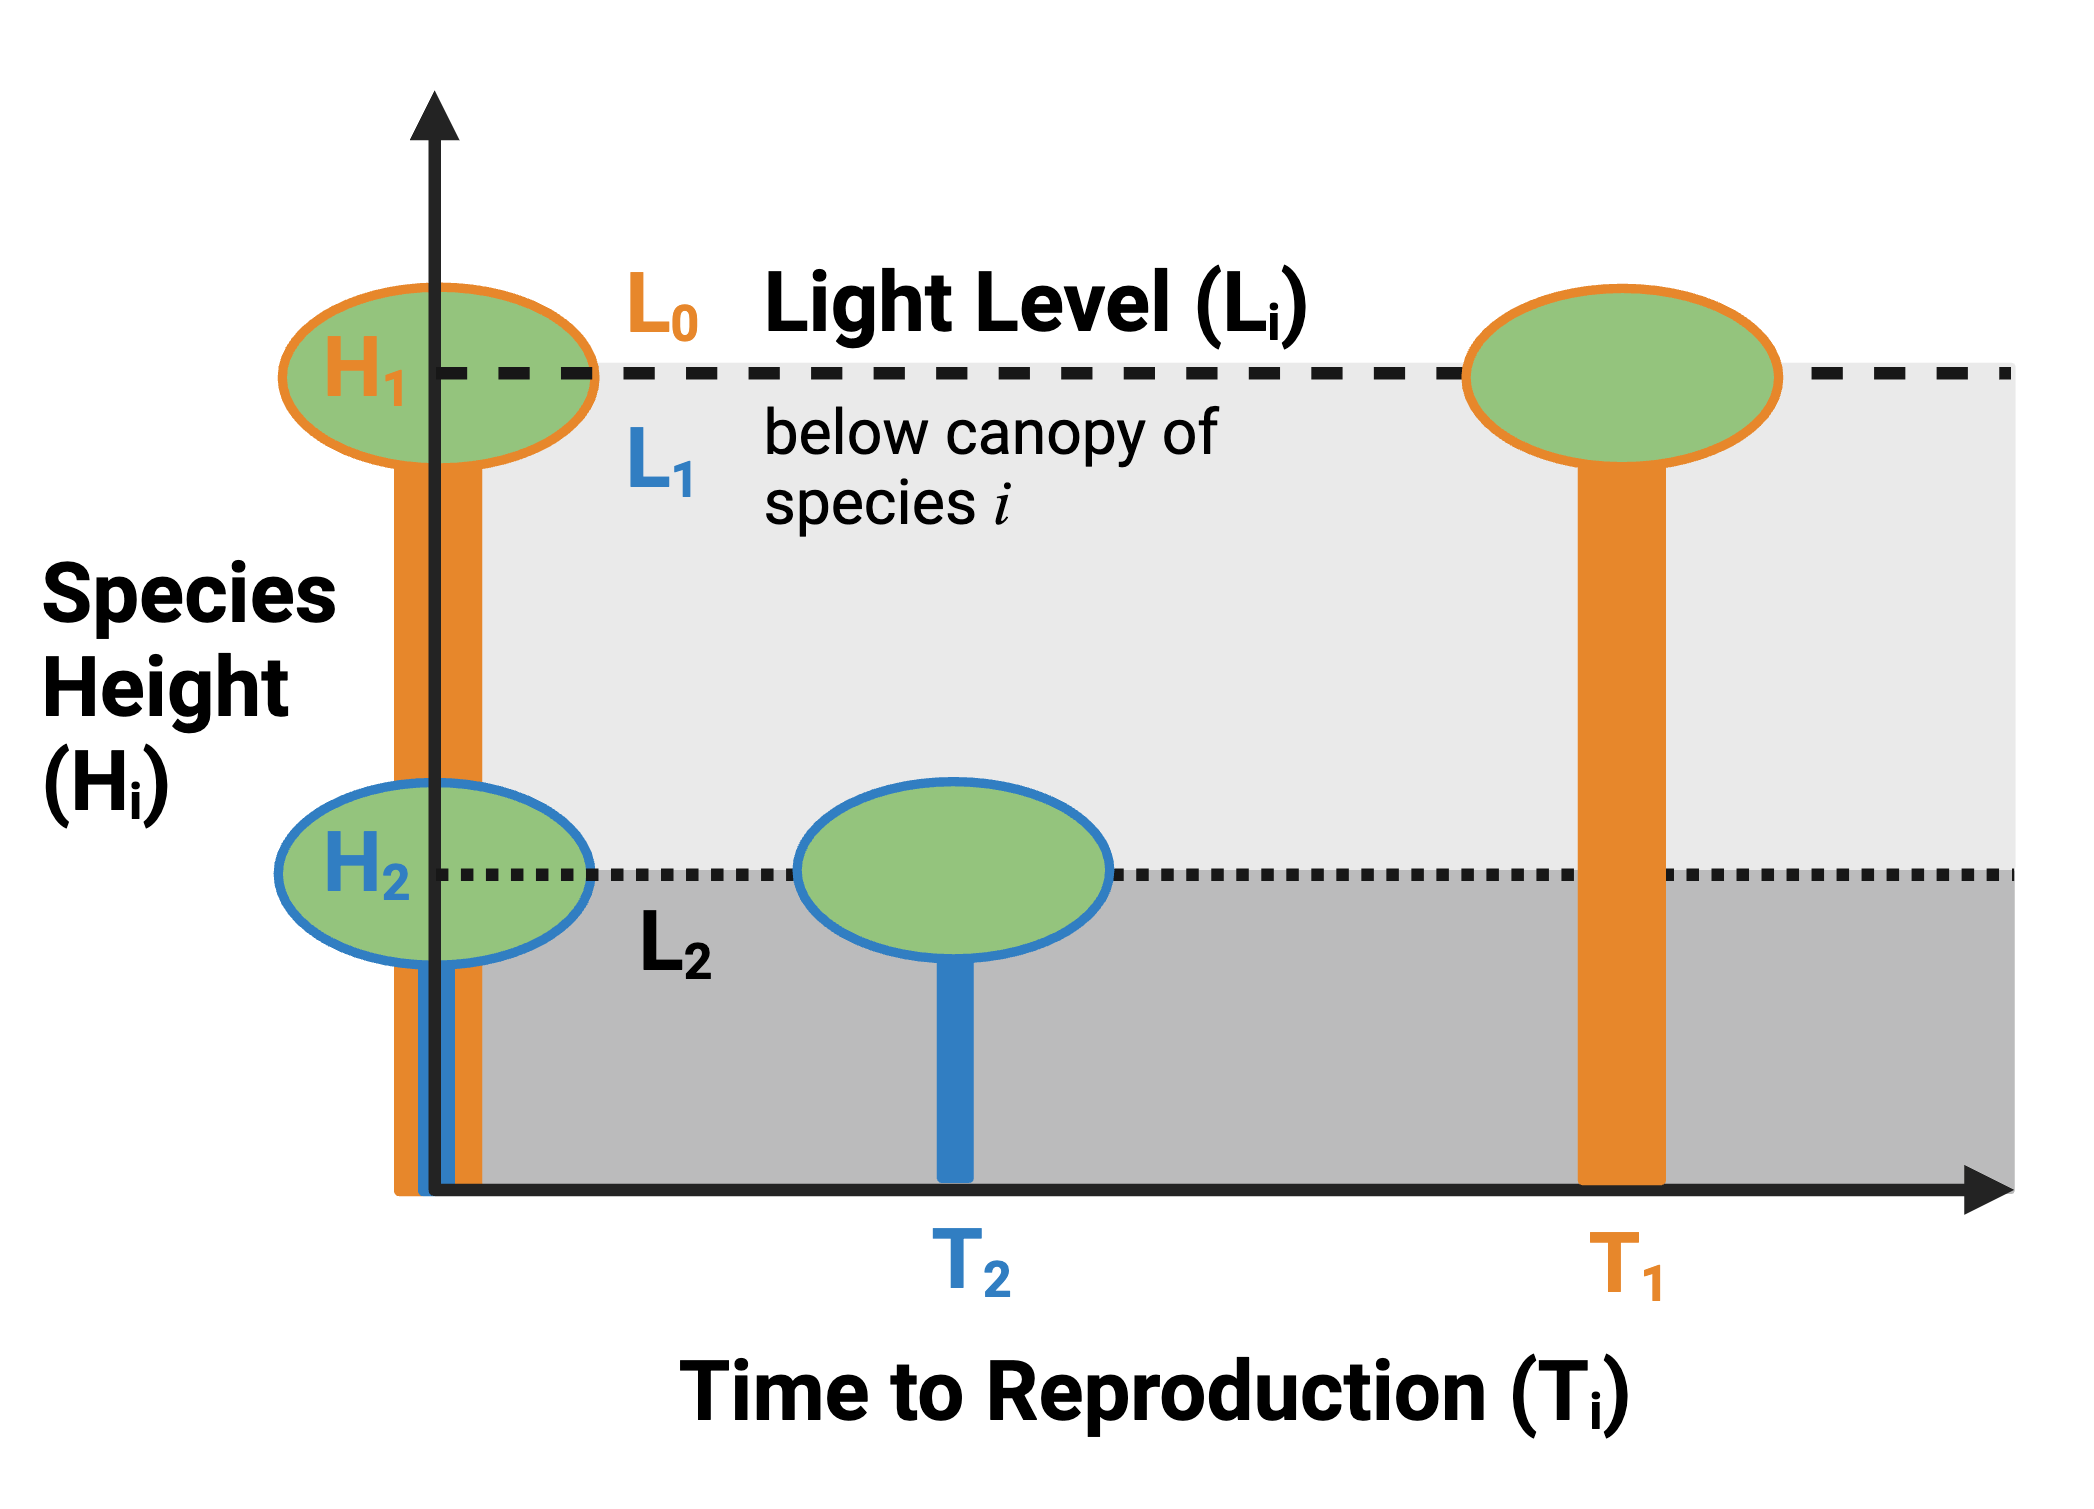
\includegraphics{/Users/ruby/Projects/shrub_model/diagrams/two_ramets_compete_for_light.png}
\caption{Diagram of the tundra ramet model of light competition.}
\end{figure}

\subsection{Ramet Allometry}\label{ramet-allometry}

Ramet biomass is related allometrically to height, via the following
powerlaw.

\[ B_i = b H_i^\beta \]

where \(b\) is a biomass conversion parameter (e.g.~wood density). For
forest tree systems from which this model draws inspiration,
\(\beta = 5\) is typical, since

\begin{align}
  B &= \text{height * basal area} \\
  & H \propto D^{1/2} \text{ and } \text{basal area} \propto D^2 \\
  & \Rightarrow B \propto D^{5/2} \text{ i.e. } B \propto H^5
\end{align}

We fix ramet crown area to be equal for all species.

\[ C_i = C_j = c, \quad \forall i,j \]

\subsection{Light Competition}\label{light-competition}

The first version of this model includes only competition for light,
assuming light extinction following Beer's law.

Definitions:

\begin{align}
& L_0 &&= 1 && \text { the total light available above the canopy of all species} \\
& L_{i-1} &&= e^{-kc\sum_{j=1}^{i-1}X_j} && \text{ the light available below canopy $i-1$, thus above canopy $i$} \\
& L_{i} &&= e^{-kc\sum_{j=1}^{i}X_j} && \text{ the light available below canopy $i$ } \\
& L_{i}^a && = L_{i-1} - L_{i}  = e^{-kc\sum_{j=1}^{i-1}X_j} (1-e^{-kcX_i}) && \text{ the light absorbed by species $i$} \\
& L_{R_i} &&= \frac{L_{i-1} - L_{i}}{X_i} && \text{ the light available to a single ramet of species } i \\
\end{align}

Each species occupies one height \(H_i\) in the canopy. The light that
reaches the canopy height of species \(i\) is set by the number of
ramets of species taller (\(j < i\)) than species \(i\). Ramets of
species \(i\) share the light that reaches their canopy equally.

The light that reaches each ramet \(R_i\) depends on:

\begin{enumerate}
\def\labelenumi{\arabic{enumi}.}
\tightlist
\item
  The light that reaches canopy \(i\), \(L_{i-1}\)
\item
  The size of canopy \(i\), i.e.~how much light all the ramets of
  species \(i\) block, \((1 - e^{-kc X_i}\))
\item
  how many ways ramets of species \(i\) need to share the captured
  light, \(X_i\).
\end{enumerate}

Each ramet of species \(i\) gets an equal ``piece of the light''
absorebed at that height level.

\subsection{Carbon Gain and Loss}\label{carbon-gain-and-loss}

Carbon gain per ramet is determined by light availability. When exposed
to a given light level (\(L_{R_i}\)), ramets gain carbon through
photosynthesis (\(A(L_{R_i})\)) and lose carbon due to respiration and
maintenance costs (\(r\)). The carbon accumulation rate of a ramet of
species \(i\) when exposed to light level \(L_{R_i}\), is given by:

\[ g_i(L_{R_i}) = A(L_{R_i})  - r\] \(A(L_{R_i})\) is a function
describing photosynthesis per ramet. For now, we assume that
photosynthesis is a linear function of light availability.

\[A(L_{R_i}) = a L_{R_i}\] where \(a\) is the rate of carbon gain per
ramet. Carbon losses \(r\) include leaf respiration and construction
costs (i.e.~1 / leaf turnover rate).

\textbf{\emph{NOTE:}} For now, we assume \(a\) and \(r\) are fixed
parameters equal for all species. Since crown area is the same across
species, I write the physiological parameters \(a\) and \(r\) to be
rates as carbon gain or loss \textbf{per ramet}. In further models, I
may rewrite to explicitly include species specific crown area. In this
case, these physiological rates would be written per unit leaf area.

\subsection{Ramet Demography}\label{ramet-demography}

Once a ramet accumulates carbon equivalent to its species-specific
biomass (\(B_i\)), it produces a full-size daughter ramet. This means
reproduction is not continuous, but pulsed at a certain interval per
species.

Based on our description of ramet allometry and physiology, we can write
an expression for the time required until reproduction (\(T_i\)),

\[ T_i = \frac{B_i}{g_i(L_{R_i})} \] At equilibrium, \(\hat T_i\) is a
fixed value for each species. This value sets the fecundity (birth rate
per unit time) of a species.

Ramets die at a constant species-specific mortality rate, \(m_i\).

\subsection{Population Dynamics}\label{population-dynamics}

In this model, we track the number of individual ramets per species per
unit area (i.e.~\(X_i(t)\) is the density of species \(i\) over time).

\[\frac{dX_i}{dt} = f_i X_i - m_i X_i = (f_i - m_i)X_i\]

At equilibrium, births and deaths exactly balance and this derivative is
zero. Because of the pulsed nature of reproduction assumed in this
clonal model, the actual expression for \(f_i\) is somewhat complicated.
To calculate equilibrium values, it's easier to consider the lifetime
reproductive success of a ramet of species \(i\).

If reproduction were continuous, we could write
\(f(i) = \frac{1}{T_i}\). However, since reproduction is pulsed, the
true value of \(f_i\) is slightly lower than this, and a somewhat
complicated ``floor'' function based on intervals of \(T_i\).

To avoid dealing with these discontinuities, it's useful to consider the
lifetime reproductive success (\(LRS\)) of each ramet, i.e.~the expected
number of offspring per ramet.

\[LRS(R_i) = \sum_{w=0}^\infty e^{-m_i T_i w}b(w) \quad \text{ where } b(w) = \begin{cases}
   0 &\text{if } w = 0 \\
   1 &\text{if } w > 0
\end{cases}\]

Note that \(e^{-m_i T_i w}\) is the probability that the ramet will
survive until age \(w\). Verbally, this means that each time the ramet
lives a time period \(T_i\), it has one daughter. The lifetime
reproductive success is the sum over all ages of the probability the
ramet lives to that age times the number of offspring it produces at
that age. When the ramet is age \(w = 0\), it has not yet reached
\(T_i\) and thus does not contribute any offspring.

If we solve \(LRS(R_i) = 1\), we get an expression that relates \(T_i\)
to mortality rate:

\[T_i = \frac{ln(2)}{m_i}\]

In words, time to reproduction at equilibrium must exactly balance the
mortality rate. Recall that we already have an expression for \(T_i\)
bulit from the physiological process of carbon accumulation to make a
baby:

\[T_i = \frac{ln(2)}{m_i} =  \frac{B_i}{g_i(L_{R_i})} \] By setting
these equal, we can solve for \(\hat L_{R_i}\), the level of light per
ramet for the system to be at equilibrium.

\[\hat L_{R_i} = \frac{1}{a} \left( \frac{m_i B_i}{ln(2) c} + r \right)\]

\section{Model Analysis}\label{model-analysis}

\subsection{Establishment Condition}\label{establishment-condition}

The biomass of a ramet increases in proportion to height to the 5th
power. This means that the taller the species, the longer it will take a
ramet to accumulate enough carbon to reproduce. We can plot the ``light
required for a species of height x'' to invade from rare, e.g.~lifetime
reproductive success \textgreater{} 0 assuming no other ramets of the
same species, as given below.

This means that the light must be AT LEAST this level in order for
species of a given height to establish.

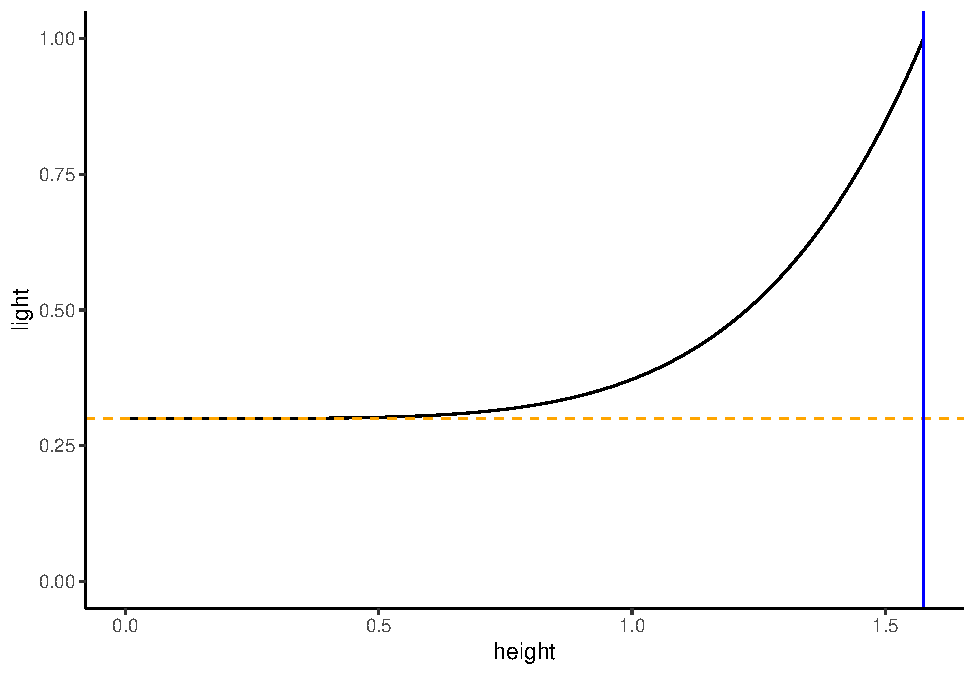
\includegraphics{ramet_model_description_files/figure-latex/unnamed-chunk-1-1.pdf}

\subsection{Equlibrium Light
Requirement}\label{equlibrium-light-requirement}

From the descirption of light competition, we have an expression for the
light available to a single ramet of species \(i\). From the demography
and physiology of the system, we know the light level required per ramet
for the system to be at equilibrium. \begin{align}
& L_{R_i} &&= \frac{L_{i-1} - L_{i}}{X_i} && \text{ the light available to a single ramet of species } i \\
& \hat L_{R_i} &&= \frac{1}{a} \left( \frac{m_i B_i}{ln(2) c} + r \right) && \text{ light requirement per ramet at equilibrium}
\end{align}

Based on our formulation of asymmetric light competition,
\(\hat L_{R_i}\) is a function of \(\hat X_j\) for \(j \leq i\). This
then gives us an implicit expression for the equilibrium density of each
species \(\hat X_i\) based on the density of taller species.

\subsection{Equilbrium Density of light extinction model w/height
reproduction
trade-off}\label{equilbrium-density-of-light-extinction-model-wheight-reproduction-trade-off}

This code randomly chooses S number of species with a trait along the
light requirement access. It then calculates the equilibrium species
density of the species. Steps for the code.

\begin{enumerate}
\def\labelenumi{\arabic{enumi}.}
\tightlist
\item
  choose number of species, S
\item
  set light extinction coefficient, k
\item
  randomly choose number of species uniformly along light requirement
  axis (u\_min to 1)
\item
  sequentially calculate equilibrium densities, from tallest species to
  shortest
\end{enumerate}

Inputs: - S : number of species in the pool (e.g.~50) - k : light
extinction coefficient

Outputs: - n: vector of equilibrium species density - u: vector
species-specific minimum light level - L: vector of light level

\subsubsection{Equilibrium density as a function of light available -
from implicit
expression}\label{equilibrium-density-as-a-function-of-light-available---from-implicit-expression}

From the implicit expression for x\_i we can solve for the equilibrium
densities of each species, based on their light requirement trait and
the densities of taller species.

The more light required, the lower the equilibrium density of the
species.
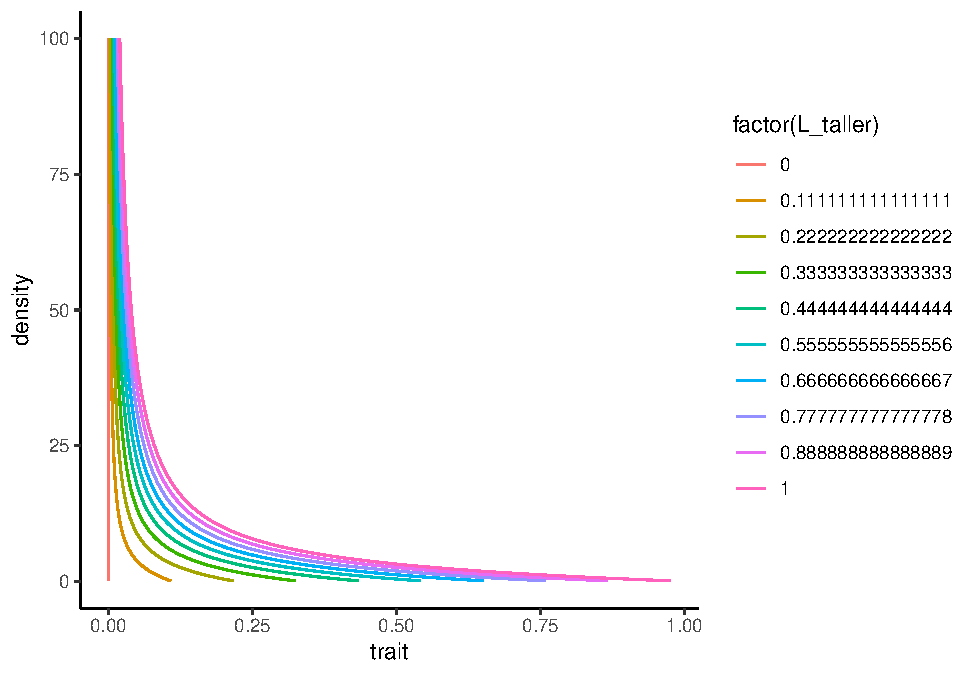
\includegraphics{ramet_model_description_files/figure-latex/unnamed-chunk-2-1.pdf}
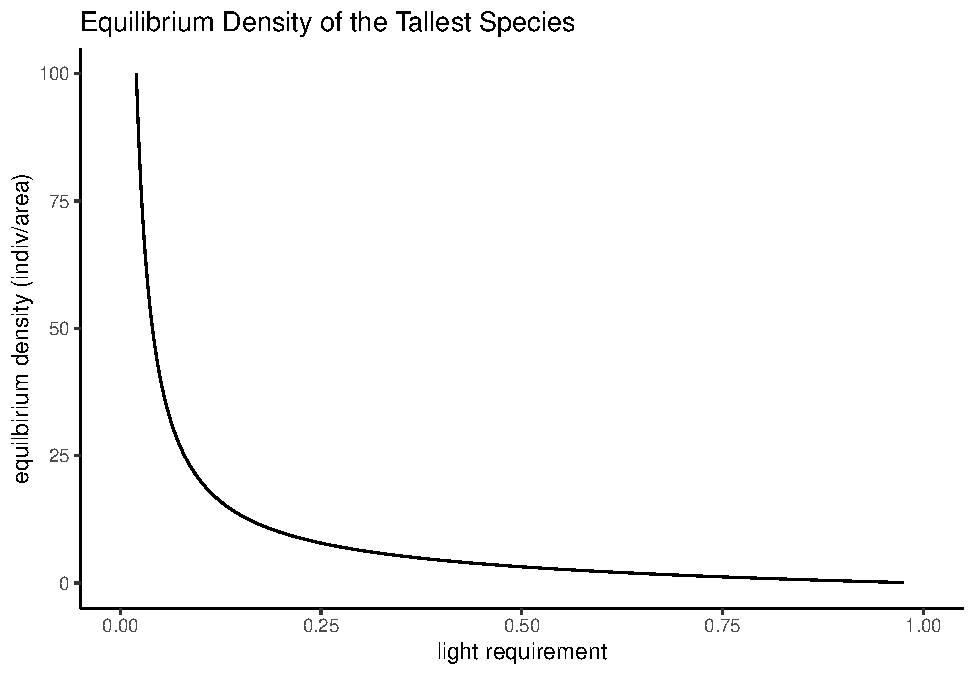
\includegraphics{ramet_model_description_files/figure-latex/unnamed-chunk-2-2.pdf}

\subsection{Equilibrium Density}\label{equilibrium-density}

\section{Model Simulations}\label{model-simulations}

\subsection{Parameters}\label{parameters}

\begin{verbatim}
## <environment: R_GlobalEnv>
\end{verbatim}

\begin{longtable}[]{@{}llrll@{}}
\toprule\noalign{}
species & parameter & value & description & unit \\
\midrule\noalign{}
\endhead
\bottomrule\noalign{}
\endlastfoot
all & a & 10.0 & rate of leaf photosynthesis & NA \\
all & r & 4.0 & rate of leaf respiration & NA \\
all & c & 20.0 & crown area & cm2 \\
all & b & 0.5 & biomass density & NA \\
all & k & 0.5 & light decay coefficient & NA \\
all & beta & 5.0 & height to mass power & NA \\
all & m & 1.0 & ramet mortality & NA \\
env & L\_above & 1000.0 & light available above & Total PAR \\
\end{longtable}

\subsubsection{Equilibrium density - sequential solution for
multispecies
community}\label{equilibrium-density---sequential-solution-for-multispecies-community}

\paragraph{Functions}\label{functions}

\subsection{Climate Change Scenarios}\label{climate-change-scenarios}

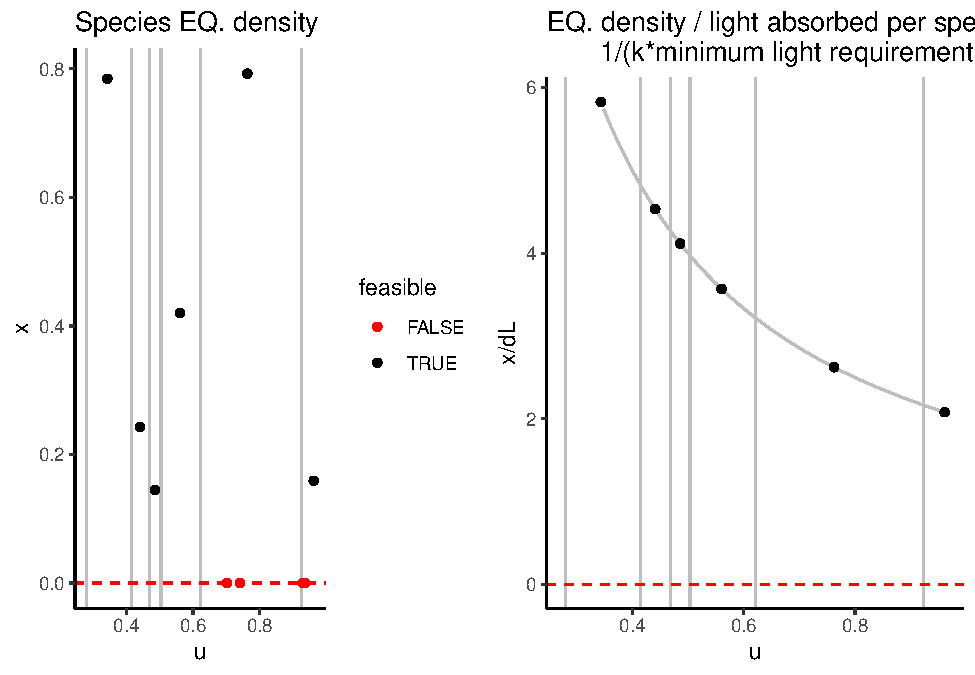
\includegraphics{ramet_model_description_files/figure-latex/unnamed-chunk-4-1.pdf}

\subsubsection{Control vs Shrubified}\label{control-vs-shrubified}

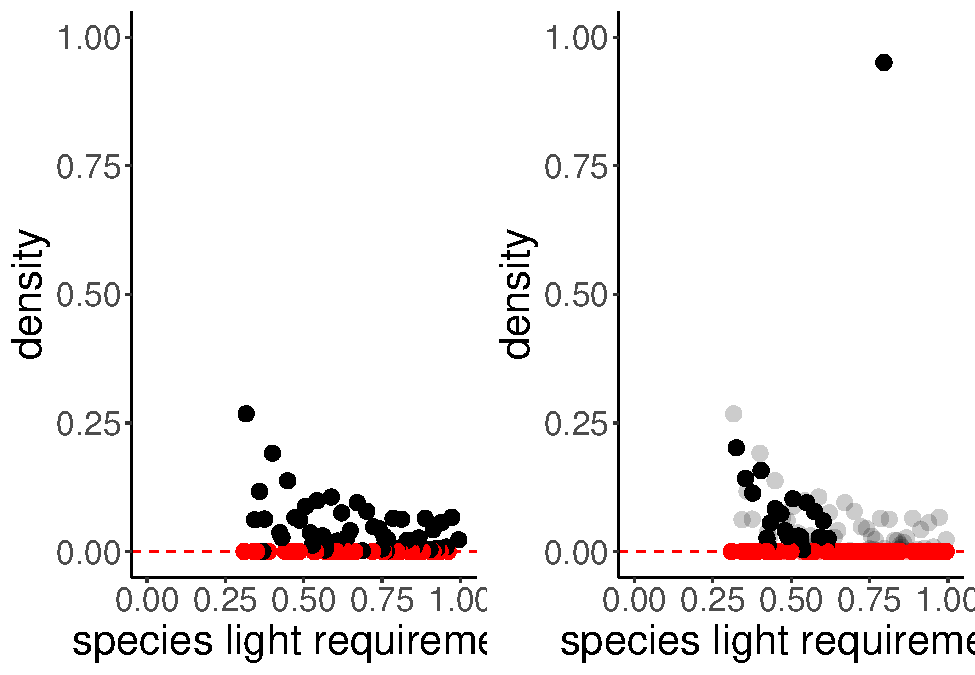
\includegraphics{ramet_model_description_files/figure-latex/unnamed-chunk-5-1.pdf}

\subsubsection{10 vs 100 species}\label{vs-100-species}

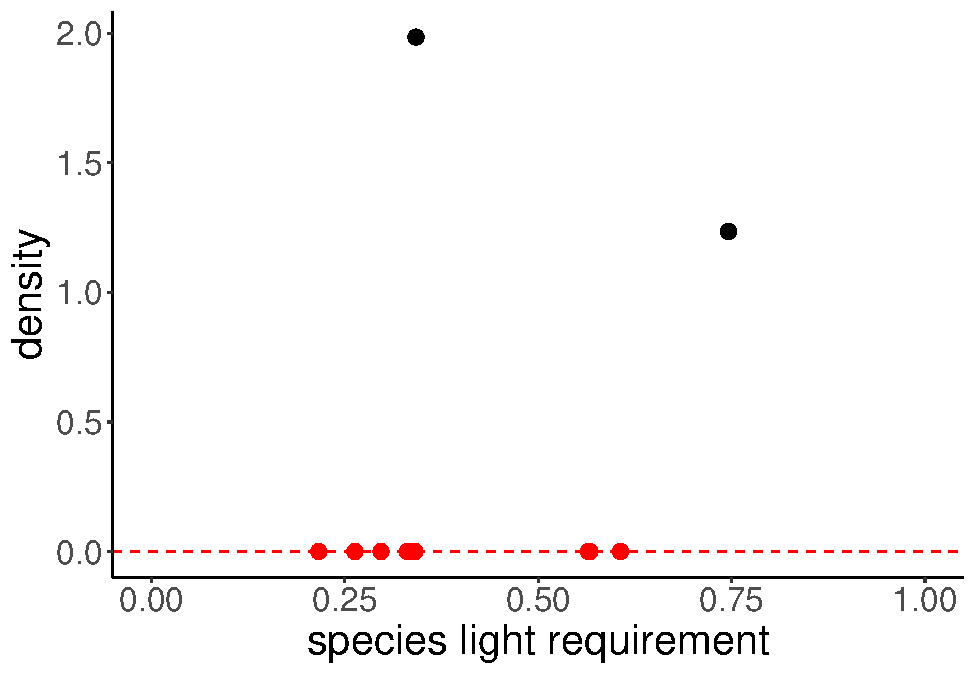
\includegraphics{ramet_model_description_files/figure-latex/unnamed-chunk-6-1.pdf}
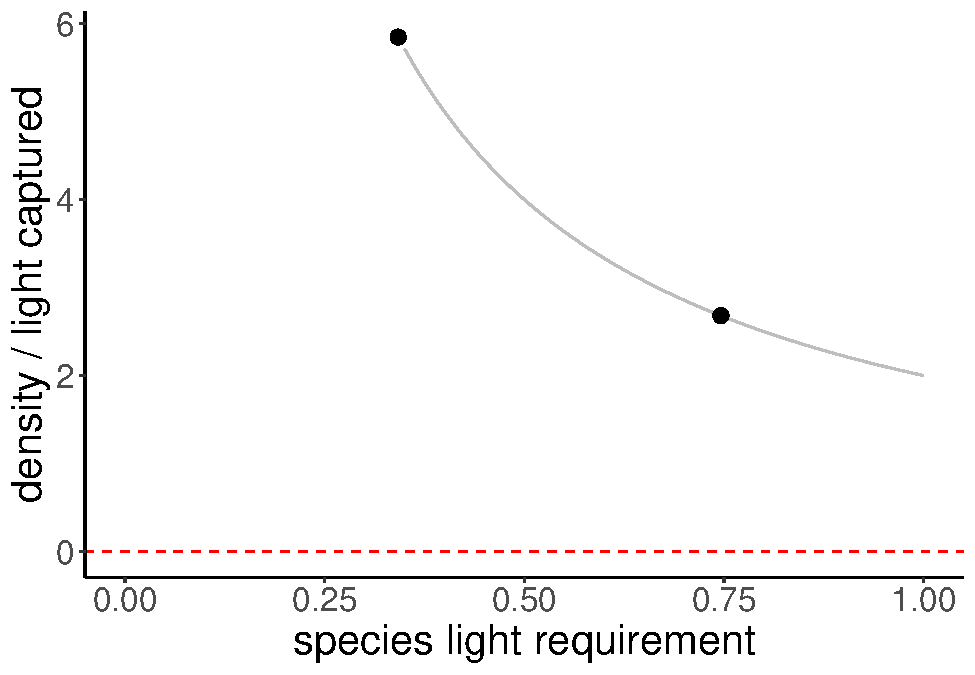
\includegraphics{ramet_model_description_files/figure-latex/unnamed-chunk-6-2.pdf}
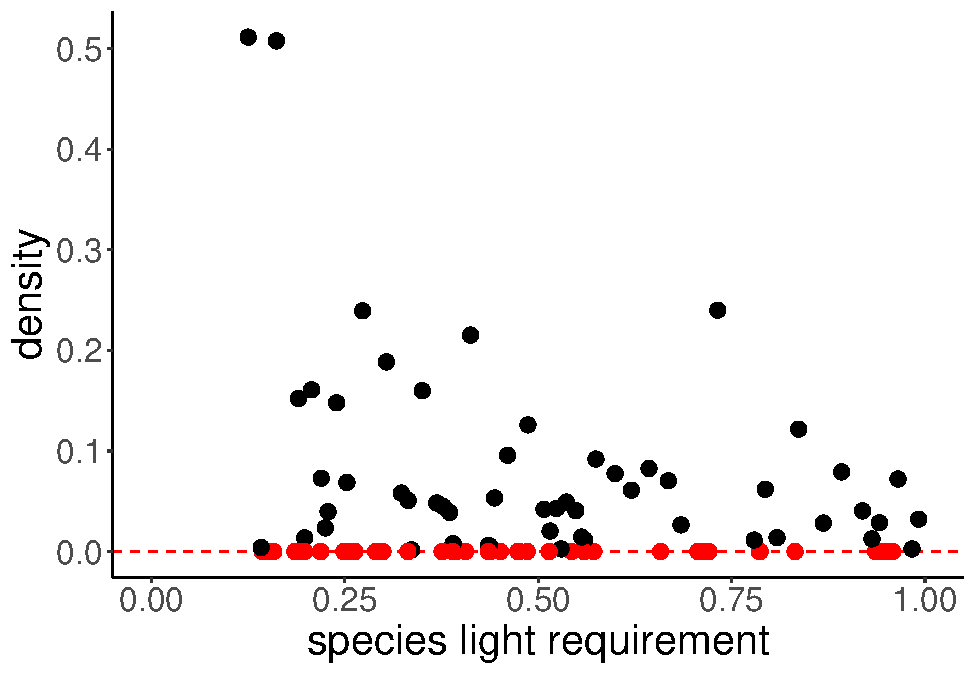
\includegraphics{ramet_model_description_files/figure-latex/unnamed-chunk-6-3.pdf}
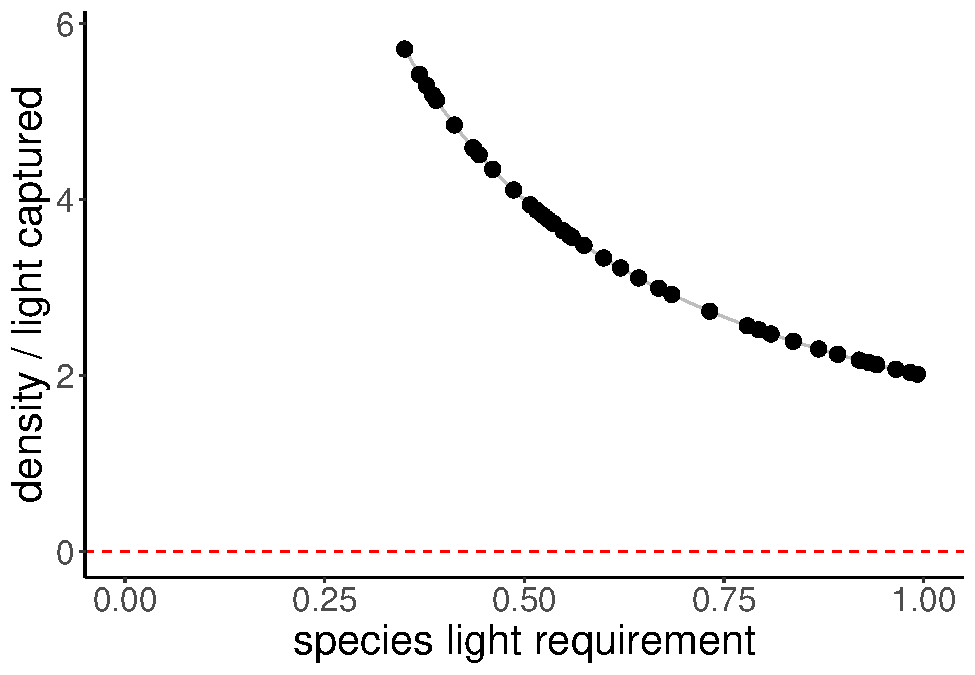
\includegraphics{ramet_model_description_files/figure-latex/unnamed-chunk-6-4.pdf}
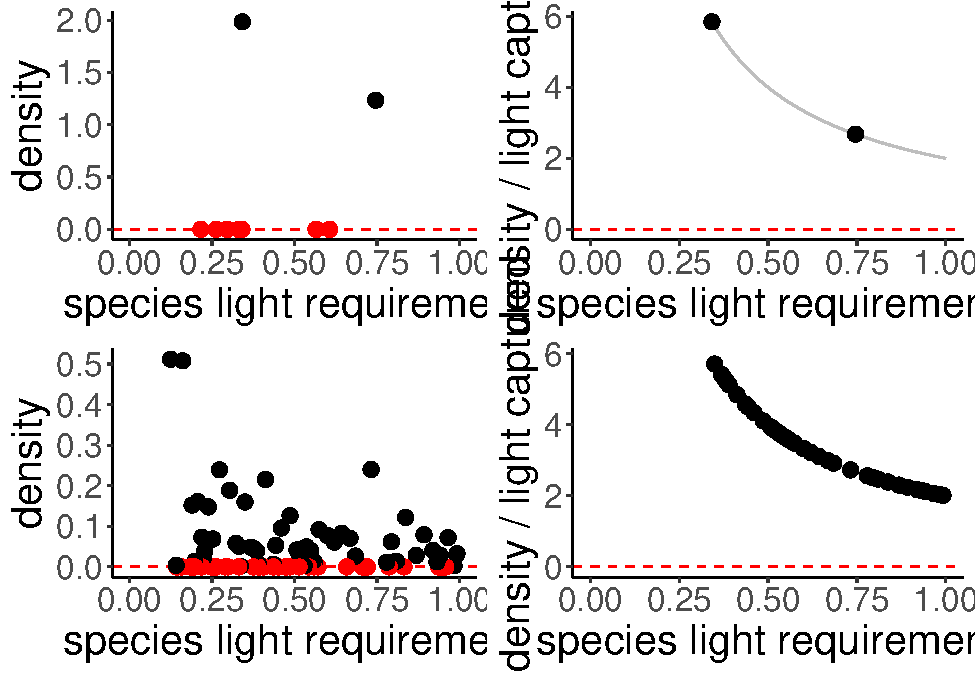
\includegraphics{ramet_model_description_files/figure-latex/unnamed-chunk-6-5.pdf}

\subsection{OTHER PLOTS}\label{other-plots}

\subsubsection{Biomass plot}\label{biomass-plot}

Here it's important that the minimum light requirement corrresponds to
an actually feasible biomass.

\subsubsection{Other scrap code}\label{other-scrap-code}

\end{document}
